% edits to do:
% make sure the references match the style instructed in the guidelines.
% references to pay attention to:
%   literature review section, line 394

\documentclass[12pt,a4paper]{article}

% ── Packages ──────────────────────────────────────────────────────────────────
\usepackage[a4paper, top=0.75in, bottom=0.75in, left=1.2in, right=1.2in]{geometry}
% times        : Times New Roman-style serif font throughout
% microtype    : subtle justification and kerning improvements
% parskip      : blank line between paragraphs instead of indentation
% setspace     : line spacing control via \setstretch
% titlesec     : custom section/subsection heading formatting
\usepackage{times}
\usepackage{microtype}
\usepackage{parskip}
\usepackage{setspace}
\usepackage{titlesec}

% maths
\usepackage{amsmath, amssymb}

% tables
\usepackage{booktabs}       % \toprule, \midrule, \bottomrule for clean tables

% figures
\usepackage{graphicx}
\usepackage{subcaption}     % side-by-side figures with \begin{subfigure}

% misc
\usepackage{hyperref}
\usepackage{enumitem}       % fine-grained list spacing control
\usepackage{xcolor}
\usepackage[authoryear]{natbib}
\usepackage[numbib, nottoc]{tocbibind}

% ── Section formatting ────────────────────────────────────────────────────────
% Sections   : large bold, horizontal rule beneath
% Subsections: normal-size bold, no rule
\titleformat{\section}{\large\bfseries}{\thesection}{1em}{}[\titlerule]
\titlespacing{\section}{0pt}{14pt}{6pt}
%                     left  before  after

\titleformat{\subsection}{\normalsize\bfseries}{\thesubsection}{1em}{}
\titlespacing{\subsection}{0pt}{10pt}{4pt}

% ── Hyperref ──────────────────────────────────────────────────────────────────
% URL colour is black by default; override per-link with \textcolor if needed
\hypersetup{
    colorlinks=true,
    linkcolor=black,
    urlcolor=black,
    pdftitle={Photon Trajectories and Optical Phenomena in Schwarzschild Spacetime: A Numerical Simulation Study},   % EDIT
}

% ── Line spacing ──────────────────────────────────────────────────────────────
% 1.0 = single spacing. Use 1.5 for draft review copies.
\setstretch{1.5}

% ══════════════════════════════════════════════════════════════════════════════
\begin{document}

% ── COVER PAGE BEGIN ──────────────────────────────────────────────────────────
% \null\vfill ... \vfill\null centres the block vertically on the page.
% \pagestyle{empty} suppresses page number on the cover.
\pagestyle{empty}
\null\vfill
\begin{center}

{\LARGE \textbf{Internship Report}}          % e.g. Internship Synopsis / Lab Report

\vspace{0.1cm}

{\LARGE \textbf{On}}

\vspace{0.1cm}

{\LARGE \textbf{Research Internship}}        % e.g. Research Internship / Course Project

\vspace{0.93cm}

{\large \bfseries Photon Trajectories and Optical Phenomena in Schwarzschild Spacetime: A Numerical Simulation Study}

\vspace{0.93cm}

{\large \textbf{Submitted by}}

{\large Aditya Pandya (23-PH-0313)}

{\large \textbf{Under the guidance of}}

{\large Dr. Pankaj Joshi}

\vspace{0.2cm}

{\large International Centre for Space and Cosmology (ICSC), Ahmedabad University}

\vspace{0.93cm}


\includegraphics[width=6cm]{images/logo.png}          % replace logo.png with your institution's logo

\vspace{0.2cm}

{\large 2023--2027}

\vspace{0.2cm}

{\large Department of Physics and Electronics}
{\large St. Xavier's College, Ahmedabad-380009}

{\large \textbf{Date of submission:} 11/05/2026.}

\end{center}
\vfill\null
\clearpage
\newpage

% ── DECLARATION ───────────────────────────────────────────────────────────────────────────

\clearpage
\pagestyle{plain}
\pagenumbering{roman} % Starts Roman numeral numbering for front matter

\begin{center}
    \Large\textbf{DECLARATION}
\end{center}

\vspace{1cm}

I, Aditya Pandya, 23-PH-0313, hereby declare that the internship report titled ``Photon Trajectories and Optical Phenomena in Schwarzschild Spacetime: A Numerical Simulation Study'', submitted to the Department of Physics and Electronics, St. Xavier's College, Ahmedabad is an original work completed by me under the guidance of Dr. Pankaj Joshi.

\vspace{0.5cm}

I hereby declare that this work is the result of my own independent effort, and I have acknowledged all materials and person/institute involved.

\vspace{3cm}

\begin{flushright}
    \rule{6cm}{0.5pt} \\ % Line for your signature
    \vspace{0.2cm}
    \textbf{Aditya Pandya} \\
    Date: 11/05/2026
\end{flushright}
\clearpage

% ═════════════════════════════════════════════════════════════════════════════════════════
\section*{Acknowledgements}
% ═════════════════════════════════════════════════════════════════════════════════════════

\vspace{\baselineskip}
I wish to express my sincere gratitude to Dr. Pankaj Joshi, Founding Director of the International Centre for Space and Cosmology (ICSC) at Ahmedabad University, for his invaluable guidance, constant encouragement, and insightful discussions throughout the duration of this research internship. His expertise in general relativity and spacetime geometry provided the intellectual foundation upon which this project was built, and his willingness to engage with both conceptual and computational challenges made the learning experience deeply rewarding.

I am grateful to the faculty of the Department of Physics and Electronics at St. Xavier’s College (Autonomous), Ahmedabad, for their academic support and for providing the institutional framework that made this internship possible. In particular, I thank the college administration for facilitating the formal collaboration with ICSC.

I also acknowledge the broader scientific community whose open-access resources were indispensable to this work: the SciPy and NumPy development teams for producing world-class numerical tools, the Matplotlib community for visualization capabilities, and the Event Horizon Telescope Collaboration for making their observational data and methodology publicly available. The interactive pedagogical materials developed by the Open Source Physics project also served as inspiration for the visualization-driven approach adopted in this study.

Finally, I thank my family and peers for their patience and support during the many long hours of debugging, derivation, and simulation that this project demanded. Their encouragement sustained me through the inevitable setbacks that accompany computational research.

\newpage

% ── TABLE OF CONTENTS ─────────────────────────────────────────────────────────────────────
\pagestyle{plain}
\tableofcontents
\clearpage

\pagenumbering{arabic} % Switch to normal numbering for the report body
\setcounter{page}{1}   % Restart at 1 for the Introduction

% ═════════════════════════════════════════════════════════════════════════════════════════
\section{Introduction}
% ═════════════════════════════════════════════════════════════════════════════════════════

Schwarzschild spacetime is the unique, exact vacuum solution to the Einstein field equations for a static, spherically symmetric mass distribution. Expressed in geometrised units ($G = c = 1$), the line element in the equatorial plane ($\theta = \pi/2$) is
\begin{equation*}
    ds^{2} = -\!\left(1 - \frac{2M}{r}\right)dt^{2}
             + \left(1 - \frac{2M}{r}\right)^{-1}dr^{2}
             + r^{2}\,d\phi^{2},
\end{equation*}
where $M$ is the gravitational mass of the central object. Photons propagate along null geodesics ($ds^{2} = 0$), and the structure of these geodesics encodes observationally significant phenomena. The effective potential for photon motion admits a local maximum at $r = 3M$, which defines the \emph{photon sphere} — an unstable circular orbit with critical impact parameter $b_{c} = 3\sqrt{3}\,M$. Photons with $b < b_{c}$ are captured, while those with $b > b_{c}$ are deflected; in the weak-field limit the deflection angle reduces to the well-known result $\Delta\phi \approx 4M/b$. These are not merely theoretical constructs: the boundary in impact parameter space between escaping and captured photons directly determines the angular radius of the black hole shadow. The shadow of the supermassive black hole M87*, imaged by the Event Horizon Telescope (EHT) in 2019, is a direct observational manifestation of precisely this physics.

The analytic framework for photon geodesics in Schwarzschild spacetime is well established, and closed-form results are available for the photon sphere radius, the critical impact parameter, and the weak-field deflection angle. However, reading these results in a textbook is not the same as building a working simulation from first principles and watching the trajectories emerge from the equations of motion. A numerical study, implemented using only standard scientific Python libraries (\texttt{NumPy}, \texttt{SciPy}, and \texttt{matplotlib}) without any pre-packaged general relativity simulation library, forces direct engagement with the physics at every step: the conserved quantities must be correctly identified, the ODE system must be properly formulated, and numerical pathologies near the photon sphere and the coordinate singularity at $r = 2M$ must be handled explicitly. This computational approach also makes phenomena such as gravitational time dilation directly visible in a way that equations alone do not convey.

This project was undertaken with the following specific objectives. First, the first-order ODE system for null geodesics in the equatorial Schwarzschild spacetime was derived from the metric, using the two conserved quantities — energy $E$ and angular momentum $L$ — that follow from the time-translation and azimuthal Killing vectors. Second, these equations were solved numerically using the RK45 adaptive integrator (\texttt{scipy.integrate.solve\_ivp}) with tight tolerances ($\texttt{rtol} = 10^{-10}$, $\texttt{atol} = 10^{-12}$), with the null invariant $g_{\mu\nu}\dot{x}^{\mu}\dot{x}^{\nu} = 0$ tracked throughout as a conservation-law check. Third, photon trajectories were classified by impact parameter $b = L/E$ into three qualitatively distinct regimes: deflection ($b > b_{c}$), capture ($b < b_{c}$), and the asymptotically critical orbit ($b \to b_{c}$) that spirals toward the photon sphere at $r = 3M$. Fourth, the effective potential $V_{\mathrm{eff}}(r) = (L^{2}/r^{2})(1 - 2M/r)$ was plotted and compared against its Newtonian counterpart to make the relativistic origin of photon capture explicit. Fifth, the numerically measured deflection angle was compared against the weak-field approximation
$\Delta\phi \approx 4M/b$ to quantify the regime of validity of that formula. Finally, a selected trajectory was animated in Schwarzschild coordinate time $t$ rather than the affine parameter $\lambda$, achieved by interpolating the spatial coordinates onto a uniform $t$-grid, so that the progressive slowdown of the photon near the horizon — the signature of gravitational time dilation as seen by a distant observer — is directly visible in the animation.


% ═════════════════════════════════════════════════════════════════════════════════════════
\section{Literature Review}
% ═════════════════════════════════════════════════════════════════════════════════════════

The theoretical foundation of this project rests on two standard graduate-level texts in general relativity. The Schwarzschild metric, its derivation as the unique spherically symmetric vacuum solution to the Einstein field equations, and the formalism of Killing vectors and conserved quantities along geodesics are treated in detail by \citet{Schutz2022} and \citet{Hobson2006}. Both texts derive the effective potential for photon orbits and establish the existence of the photon sphere at $r = 3M$ and the critical impact parameter $b_c = 3\sqrt{3}\,M$, which separates captured trajectories from escaping ones. These results form the direct theoretical basis for the ODE system integrated in this project. The purely relativistic correction term $3ML^2/r^4$ in the radial equation of motion—absent in Newtonian gravity—is what produces the maximum in $V_\text{eff}(r)$ and therefore makes photon capture physically possible; this point is discussed explicitly in \citet{Hobson2006} in the context of comparing Newtonian and relativistic orbit equations.

The numerical approach used here—Runge-Kutta integration of a first-order ODE system—is well established in the scientific computing literature. \citet{Chapra2015} provide a thorough treatment of the RK45 scheme (the Dormand-Prince variant), adaptive step-size control, and the practical problem of tolerance selection for stiff or near-singular systems. The sensitivity of photon trajectories near $b \approx b_c$ is precisely such a situation: a photon that orbits the photon sphere many times amplifies any integration error, making tight tolerances ($\texttt{rtol} = 10^{-10}$, $\texttt{atol} = 10^{-12}$) necessary rather than conservative. The use of a conserved quantity—the null invariant $g_{\mu\nu}\dot{x}^\mu\dot{x}^\nu = 0$—as a numerical sanity check is standard practice in geodesic integration, and its role as an error diagnostic is consistent with the conservation-law monitoring strategies discussed in \citet{Chapra2015}.

The simulation was implemented entirely using peer-reviewed open-source scientific Python libraries. The \texttt{solve\_ivp} integrator with the RK45 scheme is part of SciPy \citep{Virtanen2020}, array operations and data handling are performed using NumPy \citep{Harris2020}, and all visualizations—including the polar trajectory plots and the coordinate-time animation—were produced with Matplotlib \citep{Hunter2007}. Citing these as references is not a formality: each represents a substantial body of validated numerical infrastructure, and the accuracy of the simulation results depends directly on their correctness. Additional guidance on scientific visualization practices in Python was drawn from \citet{Rougier2021} and \citet{VanderPlas2016}.

While the physics of null geodesics in Schwarzschild spacetime is analytically well understood and covered in standard textbooks, there is no widely available minimal-dependency numerical implementation that simultaneously demonstrates trajectory classification by impact parameter, the effective potential with its Newtonian comparison, weak-field deflection angle verification, and gravitational time dilation as a directly visible animation—all built from first principles without pre-packaged general relativity libraries. Existing pedagogical treatments present these results analytically or through qualitative diagrams. This project fills that gap at an undergraduate level, producing a simulation where each computational step maps directly onto a physical quantity in the theory, and where phenomena such as photon capture and the black hole shadow—central to the interpretation of Event Horizon Telescope observations of M87*—emerge naturally from the numerics.

% ═════════════════════════════════════════════════════════════════════════════════════════
\section{Methodology}
% ═════════════════════════════════════════════════════════════════════════════════════════

\subsection{Theoretical Framework}

\subsubsection{Spacetime and the Schwarzschild Metric}
General relativity describes gravity not as a force, but as the curvature of spacetime caused by mass. The geometry of spacetime around a non-rotating, spherically symmetric mass $M$ is described by the \textit{Schwarzschild metric}, which gives the spacetime interval $ds^2$ between two infinitesimally separated events:

\begin{equation}
    ds^2 = -\left(1 - \frac{2M}{r}\right)c^2\,dt^2
    + \left(1 - \frac{2M}{r}\right)^{-1}dr^2
    + r^2\,d\theta^2
    + r^2\sin^2\theta\,d\phi^2
    \label{eq:schwarzschild_full}
\end{equation}

\noindent where $r$ is the radial coordinate, $t$ is coordinate time, and $\theta$, $\phi$ are the standard angular coordinates. Throughout this report, \textit{geometrized units} are used: $G = c = 1$, so that mass has units of length (specifically, $M$ is the mass of the black hole in units where $G = c = 1$). This simplifies all expressions considerably.

The factor $\left(1 - 2M/r\right)$ encodes the gravitational influence of the black hole. At $r = 2M$, this factor vanishes — this is the Schwarzschild radius, marking the \textit{event horizon}, the boundary beyond which nothing, including light, can escape.

\subsubsection{Restricting to the Equatorial Plane}
By the spherical symmetry of the Schwarzschild metric, any geodesic (the curved-spacetime generalization of a straight line, i.e., the path a freely falling particle follows) that begins in the equatorial plane $\theta = \pi/2$ with no out-of-plane velocity component will remain there for all time. Photon trajectories studied in this project are initialized in this plane, so we set $\theta = \pi/2$ (and therefore $d\theta = 0$), reducing Equation~\eqref{eq:schwarzschild_full} to:

\begin{equation}
    ds^2 = -\left(1 - \frac{2M}{r}\right)dt^2
    + \left(1 - \frac{2M}{r}\right)^{-1}dr^2
    + r^2\,d\phi^2
    \label{eq:schwarzschild_equatorial}
\end{equation}

\subsubsection{The Null Condition for Photons}
In general relativity, massive particles follow \textit{timelike} geodesics ($ds^2 < 0$), while massless particles like photons follow \textit{null} geodesics. The defining condition for a null geodesic is:

\begin{equation}
    ds^2 = 0
    \label{eq:null_condition}
\end{equation}

This is the mathematical statement that light travels along paths of zero spacetime interval. It takes the place of the familiar equation of motion for photons. Along the photon's path, all coordinates $(t, r, \phi)$ are treated as functions of an \textit{affine parameter} $\lambda$, which plays the role of a curve parameter (analogous to proper time for massive particles). Overdot notation ($\dot{~}$) will denote differentiation with respect to $\lambda$.

Applying Equation~\eqref{eq:null_condition} to the equatorial metric \eqref{eq:schwarzschild_equatorial}:

\begin{equation}
    -\left(1 - \frac{2M}{r}\right)\dot{t}^2
    + \left(1 - \frac{2M}{r}\right)^{-1}\dot{r}^2
    + r^2\dot{\phi}^2 = 0
    \label{eq:null_expanded}
\end{equation}

\subsubsection{Conserved Quantities from Killing Vectors}
A powerful feature of the Schwarzschild metric is that it has two symmetries relevant to equatorial motion: it is \textit{time-independent} (no explicit dependence on $t$) and \textit{axially symmetric} (no explicit dependence on $\phi$). In general relativity, each continuous symmetry of the metric gives rise to a conserved quantity along geodesics — this is a consequence of Noether's theorem, and the symmetry directions are formally called
\textit{Killing vectors}.

These two symmetries yield two constants of motion:

\begin{itemize}
    \item \textbf{Conserved energy} $E$, associated with time-translation
    symmetry:
    \begin{equation}
        E = \left(1 - \frac{2M}{r}\right)\dot{t}
        \label{eq:conserved_energy}
    \end{equation}

    \item \textbf{Conserved angular momentum} $L$, associated with
    rotational symmetry about the $z$-axis:
    \begin{equation}
        L = r^2\,\dot{\phi}
        \label{eq:conserved_angmom}
    \end{equation}
\end{itemize}

\noindent These can be inverted to give $\dot{t}$ and $\dot{\phi}$ in terms of $E$, $L$, and $r$:

\begin{equation}
    \dot{t} = \frac{E}{\left(1 - 2M/r\right)},
    \qquad
    \dot{\phi} = \frac{L}{r^2}
    \label{eq:tdot_phidot}
\end{equation}

\subsubsection{Deriving the Radial Equation and Effective Potential}
Substituting Equations~\eqref{eq:tdot_phidot} into the null condition~\eqref{eq:null_expanded}:

\begin{equation}
    -\frac{E^2}{\left(1 - 2M/r\right)}
    + \frac{\dot{r}^2}{\left(1 - 2M/r\right)}
    + \frac{L^2}{r^2} = 0
\end{equation}

Multiplying through by $\left(1 - 2M/r\right)$:

\begin{equation}
    -E^2 + \dot{r}^2 + \frac{L^2}{r^2}\left(1 - \frac{2M}{r}\right) = 0
\end{equation}

Rearranging:

\begin{equation}
    \dot{r}^2 = E^2 - \frac{L^2}{r^2}\left(1 - \frac{2M}{r}\right)
    \label{eq:rdot_squared}
\end{equation}

This has the structure of an energy conservation equation. Defining the \textit{effective potential}:

\begin{equation}
    V_\text{eff}(r) = \frac{L^2}{r^2}\left(1 - \frac{2M}{r}\right)
    = \frac{L^2}{r^2} - \frac{2ML^2}{r^3}
    \label{eq:veff}
\end{equation}

Equation~\eqref{eq:rdot_squared} becomes the familiar-looking:

\begin{equation}
    \dot{r}^2 + V_\text{eff}(r) = E^2
    \label{eq:energy_conservation}
\end{equation}

The photon can only exist at radii where $V_\text{eff}(r) \leq E^2$; wherever $V_\text{eff}(r) > E^2$, the right-hand side would be negative, which is impossible for a real $\dot{r}$. These are classical turning points.

\subsubsection{The Impact Parameter and Geometry of Scattering}
It is convenient to factor out $E^2$ and define the \textit{impact parameter}:

\begin{equation}
    b \equiv \frac{L}{E}
    \label{eq:impact_parameter}
\end{equation}

Geometrically, $b$ is the perpendicular distance from the black hole to the incoming photon's asymptotic trajectory — the ``aim'' of the photon. Equation~\eqref{eq:rdot_squared} then becomes:

\begin{equation}
    \dot{r}^2 = E^2\left[1 - \frac{b^2}{r^2}\left(1 - \frac{2M}{r}\right)\right]
    \label{eq:rdot_b}
\end{equation}

and the trajectory's shape is determined entirely by $b$: photons with the same $b$ trace the same path in space, regardless of their individual $E$ and $L$.

\subsubsection{The Photon Sphere and Critical Impact Parameter}
To find circular photon orbits, we require both $\dot{r} = 0$ and $\ddot{r} = 0$ simultaneously — the photon must be at a turning point with zero radial acceleration. Differentiating Equation~\eqref{eq:energy_conservation} with respect to $\lambda$:

\begin{equation}
    2\dot{r}\,\ddot{r} = -V_\text{eff}'(r)\,\dot{r}
    \implies
    \ddot{r} = -\frac{1}{2}V_\text{eff}'(r)
    \label{eq:rdotdot}
\end{equation}

Setting $\dot{r} = 0$ and $\ddot{r} = 0$ requires $V_\text{eff}'(r) = 0$:

\begin{equation}
    \frac{d}{dr}\left[\frac{L^2}{r^2} - \frac{2ML^2}{r^3}\right]
    = -\frac{2L^2}{r^3} + \frac{6ML^2}{r^4} = 0
\end{equation}

Solving:

\begin{equation}
    r_\text{ph} = 3M
    \label{eq:photon_sphere}
\end{equation}

This is the \textit{photon sphere}: a spherical surface at $r = 3M$ on which photons can orbit the black hole in unstable circular orbits. It is unstable because any small perturbation causes the photon to either spiral inward and fall into the black hole, or spiral outward and escape to infinity.

Evaluating $V_\text{eff}$ at $r = 3M$ and setting it equal to $E^2$ gives the \textit{critical impact parameter}:

\begin{equation}
    b_c = 3\sqrt{3}\,M
    \label{eq:bcrit}
\end{equation}

This is the threshold that separates two qualitatively different photon trajectories:
\begin{itemize}
    \item $b < b_c$: the photon crosses the event horizon and is captured.
    \item $b > b_c$: the photon is deflected but escapes to infinity.
    \item $b = b_c$: the photon asymptotically approaches the photon sphere
    and orbits it indefinitely (in the idealized case).
\end{itemize}

\subsubsection{Physical Meaning of the Relativistic Correction Term}
From Equation~\eqref{eq:rdotdot}, the radial acceleration of the photon is:

\begin{equation}
    \ddot{r} = \frac{L^2}{r^3} - \frac{3ML^2}{r^4}
    \label{eq:rdotdot_explicit}
\end{equation}

The first term, $L^2/r^3$, is the centrifugal repulsion: it pushes the photon outward, and has a direct analog in Newtonian mechanics. In Newtonian gravity, light is not deflected toward mass in this way, and this centrifugal term alone would be the entire story.

The second term, $-3ML^2/r^4$, has no Newtonian counterpart. It is a purely relativistic correction that acts as an additional \textit{inward} pull, growing faster than the centrifugal term as $r$ decreases. This term is responsible for the photon sphere: at $r = 3M$, these two terms exactly balance ($\ddot{r} = 0$). At smaller radii, the relativistic term dominates and the photon is pulled inexorably inward. This term is the mechanism by
which strong gravity can bend and trap light — an effect entirely absent from Newtonian gravity.

\subsubsection{The First-Order ODE System}
The equations above are cast into a first-order system suitable for numerical integration. Introducing the state vector $(t,\, r,\, \dot{r},\, \phi)$, the equations of motion are:

\begin{align}
    \frac{dt}{d\lambda} &= \frac{E}{1 - 2M/r}
    \label{eq:ode_t}\\[6pt]
    \frac{dr}{d\lambda} &= \dot{r}
    \label{eq:ode_r}\\[6pt]
    \frac{d\dot{r}}{d\lambda} &= \frac{L^2}{r^3} - \frac{3ML^2}{r^4}
    \label{eq:ode_rdot}\\[6pt]
    \frac{d\phi}{d\lambda} &= \frac{L}{r^2}
    \label{eq:ode_phi}
\end{align}

Equations~\eqref{eq:ode_t} and \eqref{eq:ode_phi} follow directly from Equation~\eqref{eq:tdot_phidot}. Equation~\eqref{eq:ode_rdot} is the radial equation of motion derived in~\eqref{eq:rdotdot_explicit}. The sign of $\dot{r}$ at the initial step is chosen to match the photon's inward or outward initial direction.

This system was integrated numerically using the RK45 (Dormand-Prince) adaptive Runge-Kutta method via \texttt{scipy.integrate.solve\_ivp}, with absolute and relative tolerances of $10^{-10}$ to ensure accuracy near the critical impact parameter, where trajectories are exponentially sensitive to initial conditions. The simulation is terminated when $r \leq 2.05M$ (photon absorbed) or $r$ exceeds a specified outer boundary
(photon escapes).

As a numerical sanity check, the null invariant $g_{\mu\nu}\dot{x}^\mu\dot{x}^\nu = 0$ was monitored throughout each integration. Any significant departure from zero indicates numerical error.

\subsection{Numerical Implementation}

\label{subsec:numerical_implementation}

The equations of motion derived in the previous subsection include a second-order ODE for $r(\lambda)$ and two first-order equations for $t(\lambda)$ and $\phi(\lambda)$ obtained from the conserved quantities. Before passing these to a numerical solver, they must be rewritten entirely in first-order form, because standard ODE integrators require the system in the form $\dot{\mathbf{y}} = \mathbf{f}(\lambda,\,\mathbf{y})$.

\subsubsection{State Vector}
The integration state vector is
\begin{equation}
    \mathbf{y}(\lambda) = \bigl(t,\; r,\; \dot{r},\; \phi\bigr),
    \label{eq:state_vector}
\end{equation}
where dots denote derivatives with respect to the affine parameter $\lambda$. Each component has a specific role. $t$ is the coordinate time as measured by a distant stationary observer; it is tracked here because, in the animation, the trajectory is later re-parameterised onto a uniform $t$-grid to make gravitational time dilation visible. $r$ is the radial coordinate and is the primary spatial degree of freedom. $\dot{r}$ must be carried as a separate variable because the radial equation is second-order: introducing $\dot{r}$ explicitly converts one second-order ODE into two coupled first-order ODEs, which the solver can integrate directly. $\phi$ is the azimuthal angle, which accumulates monotonically throughout the trajectory and determines the total angular deflection.

The four first-order equations that define $\dot{\mathbf{y}}$ are

\begin{align}
    \dot{t}    &= \frac{E}{\displaystyle 1 - \frac{2M}{r}},
    \label{eq:tdot} \\[6pt]
    \dot{r}    &= \dot{r}
    \qquad \text{(propagated as an independent variable)},
    \label{eq:rdot_prop} \\[6pt]
    \ddot{r}   &= -\frac{L^{2}}{r^{3}} + \frac{3ML^{2}}{r^{4}},
    \label{eq:rddot} \\[6pt]
    \dot{\phi} &= \frac{L}{r^{2}},
    \label{eq:phidot}
\end{align}

\noindent
where $E$ and $L$ are the conserved energy and angular momentum, fixed at the start of the integration by the photon's initial conditions.

\subsubsection{Choice of Integrator}
The system was solved using \texttt{scipy.integrate.solve\_ivp} with the \texttt{RK45} method \citep{Virtanen2020}, which implements the Dormand--Prince fourth-order Runge--Kutta scheme with a fifth-order error estimate used to control the step size adaptively.

The key advantage of an adaptive integrator over a fixed-step one is that the step size automatically shrinks in regions where the solution changes rapidly — such as near the photon sphere at $r = 3M$ — and expands again in calmer regions far from the black hole. A fixed step size would have to be chosen small enough to handle the worst-case region everywhere, making the computation unnecessarily slow. The adaptive scheme achieves the same accuracy at a fraction of the computational cost.

\subsubsection{Tolerance Justification}
The accuracy of each integration step is controlled by two parameters: the relative tolerance \texttt{rtol} and the absolute tolerance \texttt{atol}. A step is accepted when its estimated local error $\varepsilon$ satisfies
\begin{equation}
    \varepsilon \;\leq\; \texttt{atol} \;+\; \texttt{rtol}\times|\mathbf{y}|.
    \label{eq:error_condition}
\end{equation}
In this simulation, the tolerances were set to
\begin{equation}
    \texttt{rtol} = 10^{-10}, \qquad \texttt{atol} = 10^{-12},
    \label{eq:tol_values}
\end{equation}
which are several orders of magnitude tighter than the \texttt{solve\_ivp} defaults
($\texttt{rtol} = 10^{-3}$, $\texttt{atol} = 10^{-6}$).

The reason is the extreme sensitivity of photon trajectories near the critical impact parameter $b \approx b_c = 3\sqrt{3}\,M$. A photon with $b$ only marginally above $b_c$ will orbit the photon sphere at $r = 3M$ many times before finally escaping; a photon with $b$ only marginally below $b_c$ will spiral inward and be captured. These two outcomes are separated by an exponentially thin boundary in impact-parameter space. Near this boundary, a small numerical error in $r$ — one that is harmless for a trajectory that escapes immediately — is amplified with each successive orbit, and can force the photon into the wrong regime entirely. With default tolerances, near-critical trajectories showed significant drift in the conserved quantities $E$ and $L$, which are exact constants of the motion and should not change. Tightening to the values in Equation~(\ref{eq:tol_values}) suppressed this drift to an acceptable level and produced consistent, reproducible orbit counts.

\subsubsection{Termination: Event Functions}
Two terminal event functions were registered with \texttt{solve\_ivp} to stop the integration automatically, rather than letting it run to a fixed affine parameter.

\begin{enumerate}
    \item \textbf{Capture event.} Integration halts when $r$ falls to $2.05\,M$.
    The Schwarzschild horizon is located at $r = 2M$, where the metric coefficient
    $g_{tt} = 1 - 2M/r$ vanishes. This causes the right-hand side of
    Equation~(\ref{eq:tdot}) to diverge, breaking down the coordinate description.
    Setting the threshold at $r = 2.05\,M$ stops the integrator just outside this
    singular region, before any metric component diverges. Any photon reaching this
    radius is classified as captured.

    \item \textbf{Escape event.} Integration halts when $r$ exceeds a large cutoff
    $r_\mathrm{max}$, chosen far enough from the black hole that spacetime is
    effectively flat there. A photon reaching $r_\mathrm{max}$ is classified as having
    escaped, and its asymptotic angular position is used to compute the deflection
    angle $\Delta\phi$.
\end{enumerate}

Both events are specified with a crossing direction so that only a genuine infall or escape triggers the condition, not a momentary approach followed by a turnaround.

\subsubsection{Numerical Sanity Check: the Null Invariant}
Photons travel along null geodesics, which by definition satisfy $ds^{2} = 0$ everywhere along the path. In terms of the four-velocity components $\dot{x}^{\mu}$, this null condition reads
\begin{equation}
    g_{\mu\nu}\,\dot{x}^{\mu}\dot{x}^{\nu} = 0.
    \label{eq:null_invariant}
\end{equation}
Expanding for the Schwarzschild metric in the equatorial plane gives
\begin{equation}
    -\!\left(1 - \frac{2M}{r}\right)\dot{t}^{\,2}
    +\left(1 - \frac{2M}{r}\right)^{\!-1}\!\dot{r}^{\,2}
    + r^{2}\dot{\phi}^{\,2} = 0.
    % \label{eq:null_expanded}
\end{equation}

Since $\dot{t}$ and $\dot{\phi}$ are evaluated analytically from the conserved quantities $E$ and $L$ at each step (Equations~\ref{eq:tdot} and \ref{eq:phidot}), the null invariant in Equation~(\ref{eq:null_expanded}) is effectively a check on the accuracy of $\dot{r}$ alone — the only quantity the integrator evolves directly. In a well-resolved integration it should remain zero to within the specified tolerances. Any noticeable departure from zero indicates that numerical errors have grown large enough to violate this fundamental physical constraint, signalling that the tolerances must be tightened or the step size reduced.

In practice this check was indispensable during development: it was the drift in $g_{\mu\nu}\dot{x}^{\mu}\dot{x}^{\nu}$ away from zero, observed with default solver tolerances, that first revealed the integrator was insufficiently accurate for near-critical trajectories and motivated the tighter settings in Equation~(\ref{eq:tol_values}).

\subsection{Trajectory Classification}

A central goal of this project was to understand how a photon's trajectory near a black hole depends on a single parameter: the \textit{impact parameter}, $b = L/E$. Here, $L$ is the photon's angular momentum and $E$ is its energy --- both constants of motion along any geodesic. Physically, $b$ measures how ``far off-centre'' the photon is headed relative to the black hole; a photon aimed directly at the black hole has $b = 0$, while one passing far away has a large $b$.

\subsubsection{The Critical Impact Parameter}
Not all photons that pass near the black hole are captured. General relativity predicts the existence of a \textit{photon sphere} at $r = 3M$ --- a radius at which gravity is exactly strong enough to hold a photon in an unstable circular orbit. This gives rise to a critical impact parameter,
\begin{equation}
    b_c = 3\sqrt{3}\, M \approx 5.196\, M,
    \label{eq:bc}
\end{equation}
which acts as a sharp boundary between qualitatively different photon fates. To understand why this threshold exists, it helps to think in terms of an effective potential. The radial motion of a photon obeys an energy-conservation-like equation,
\begin{equation}
    \dot{r}^2 = E^2 - V_\mathrm{eff}(r), \qquad
    V_\mathrm{eff}(r) = \frac{L^2}{r^2}\left(1 - \frac{2M}{r}\right),
    \label{eq:veff}
\end{equation}
where the dot denotes differentiation with respect to the affine parameter $\lambda$. $V_\mathrm{eff}$ has a single maximum at $r = 3M$, and whether the photon has enough ``energy'' to overcome this barrier --- or equivalently, whether $b$ exceeds $b_c$ --- determines the trajectory type entirely.

\subsubsection{Three Qualitatively Distinct Orbit Types}
Sweeping the impact parameter over a range of values revealed three distinct classes of photon trajectory:

\begin{enumerate}

    \item \textbf{Deflection ($b > b_c$).} The photon approaches the black hole, curves toward it due to gravity, but has sufficient angular momentum to escape back to large $r$. The trajectory is bent by an angle $\Delta\phi$ relative to the straight-line path it would have followed in flat spacetime. In this simulation, the lensing case was represented by $b = 8.0\,M$.

    \item \textbf{Critical spiral ($b \to b_c$).} When $b$ is tuned very close to $b_c$  (here, $b = 1.001\,b_c$), the photon's effective energy nearly matches the peak of $V_\mathrm{eff}$. It asymptotically approaches the photon sphere at $r = 3M$, winding around the black hole many times before eventually escaping or being captured depending on which side of $b_c$ it falls. This case required significantly tighter numerical tolerances (relative tolerance $\mathrm{rtol} = 10^{-10}$, absolute tolerance $\mathrm{atol} = 10^{-12}$), because small integration errors near the unstable equilibrium grow exponentially.

    \item \textbf{Capture ($b < b_c$).} The photon does not have enough angular momentum to
    overcome the effective potential barrier, so $\dot{r}^2$ cannot remain positive all the way out, and the photon falls inward past the event horizon at $r = 2M$ and is absorbed by the black hole. The capture case in this simulation used $b = 4.0\,M$. Integration was terminated at $r = 2.05\,M$ to avoid the coordinate singularity at the Schwarzschild horizon.

\end{enumerate}

Figure~\ref{fig:polar_trajectories} shows the polar-coordinate trajectories for all three representative cases. The photon sphere and event horizon are overlaid for reference.

\subsubsection{Deflection Angle Extraction and Comparison with the Weak-Field Formula}
For photons that escape ($b > b_c$), the net bending of the trajectory can be quantified by the deflection angle $\Delta\phi$. To extract it numerically, each photon was launched from
$r_0 = 1000\,M$ and the integration was terminated when it returned to $r = 1000\,M$ on the
other side. If spacetime were flat, the photon would trace a straight line and $\phi$ would
change by exactly $\pi$ radians from start to finish. Any excess is the gravitational deflection:
\begin{equation}
    \Delta\phi = \phi_\mathrm{final} - \pi.
    \label{eq:dphi_extract}
\end{equation}
This procedure was repeated for 60 values of $b$ uniformly spaced between $1.01\,b_c$ and $20\,M$. The large starting and ending radius ($1000\,M$) was chosen deliberately: at smaller radii, the photon's path is already noticeably curved at its start and end points, which would contaminate the deflection angle estimate.

The numerical results were compared against the standard weak-field (small-angle) prediction from General Relativity,
\begin{equation}
    \Delta\phi \approx \frac{4M}{b},
    \label{eq:wf}
\end{equation}
which is derived by treating the gravitational field as a small perturbation of flat spacetime.
This approximation holds when $b \gg M$. As $b$ decreases toward $b_c$, the photon passes much closer to the black hole where spacetime curvature is strong, and the weak-field formula is expected to underestimate the true deflection significantly. Figure~\ref{fig:deflection} shows this comparison: at large $b$, the numerical and analytic curves agree closely, but they diverge as $b \to b_c$, where $\Delta\phi$ diverges logarithmically --- a signature of the photon winding multiple times around the photon sphere.

\subsection{Animation and Coordinate-Time Reparameterization}

The numerical integrator advances the photon's trajectory using an \textit{affine parameter} $\lambda$ as its independent variable. The affine parameter is not a physical clock---it is simply a convenient mathematical label that increases smoothly along the photon's path, chosen so that the geodesic equations take a clean form. Because $\lambda$ has no direct physical meaning to an outside observer, an animation that steps frame-by-frame in  $\lambda$ would look arbitrary: the photon would appear to speed up and slow down in ways that reflect nothing real.

A more physically meaningful choice of independent variable is the \textit{coordinate time} $t$, which corresponds to the time recorded by a stationary clock located very far from the black hole---effectively, the time measured by an outside observer watching the animation. When the simulation is expressed in terms of $t$, a relativistic effect known as gravitational time dilation becomes directly visible: as a photon approaches the event horizon at $r = 2M$, the rate at which coordinate time advances \textit{per unit of affine parameter} diverges. This follows directly from the conserved energy. Since $E = (1 - 2M/r)\,\dot{t}$, one has

\begin{equation}
    \frac{dt}{d\lambda} = \frac{E}{1 - 2M/r},
\end{equation}

\noindent which grows without bound as $r \to 2M$. Physically, this means that to the outside observer, the photon appears to slow down and asymptotically freeze at the horizon---a signature of gravitational time dilation made directly observable in the animation.

\subsubsection{Reparameterization Procedure}
The raw integration output consists of arrays $r(\lambda)$, $\phi(\lambda)$, and $t(\lambda)$ sampled on the dense, adaptive grid that \texttt{solve\_ivp} chose internally. Since $t(\lambda)$ is a monotonically increasing (though non-uniform) function of $\lambda$, the trajectory can be re-expressed as a function of $t$ by inversion: given $t(\lambda)$, one obtains $r(t)$ and $\phi(t)$ by interpolation.

In practice, this was implemented using \texttt{scipy.interpolate.interp1d}. A uniform coordinate-time grid

\begin{equation}
    t_k = \frac{k}{N} \, t_{\max}, \quad k = 0, 1, \ldots, N-1,
\end{equation}

\noindent with $N = 600$ frames and $t_{\max} = 120M$, was constructed to serve as the shared time axis for all three photons in the animation. For each trajectory, the raw $(t, r)$ and $(t, \phi)$ pairs from the integrator were passed to \texttt{interp1d}, producing callable functions $r(t)$ and $\phi(t)$ that were then evaluated at every $t_k$.

Two practical complications arose in this step.

\begin{enumerate}
    \item \textbf{Horizon cutoff for captured photons.} For impact parameters $b < b_c$, the photon eventually approaches $r = 2M$, where Equation~\eqref{eq:tdot} diverges. Numerically, $t(\lambda)$ grows extremely rapidly near the end of such a trajectory, causing interpolation artifacts. To avoid this, the last $2\%$ of data points were discarded before constructing the interpolant, keeping the trajectory comfortably away from the divergence.

    \item \textbf{Freezing at the endpoint.} Once a photon has been captured or has escaped beyond the outer boundary, the global animation time $t_k$ may continue to advance beyond the photon's individual trajectory data. The \texttt{interp1d} call was configured with \texttt{bounds\_error=False} and \texttt{fill\_value} set to the photon's last known position, so that it simply freezes in place for the remainder of the animation rather than producing errors or extrapolated nonsense.
\end{enumerate}

Finally, to make the three photons approach from visually distinct directions, their azimuthal coordinates were offset by $\Delta\phi = 0$, $2\pi/3$, and $4\pi/3$ respectively. Cartesian coordinates $(x, y) = r(\cos\phi,\, \sin\phi)$ were computed at each frame and passed to \texttt{matplotlib.animation.FuncAnimation}, which rendered the result as a GIF. The outcome is that the captured photon visibly decelerates and stalls near the horizon while the lensed photon sweeps smoothly around and escapes---coordinate time making the physics directly observable.

% ═════════════════════════════════════════════════════════════════════════════════════════
\section{Results and Findings}
% ═════════════════════════════════════════════════════════════════════════════════════════

The simulation was run for three representative photon trajectories, an effective potential analysis, a deflection angle comparison, and a numerical accuracy check. Each is presented below.

\subsection{Photon Trajectories}

Three distinct classes of photon trajectory exist in Schwarzschild spacetime, determined entirely by the impact parameter $b$ relative to the critical value $b_c = 3\sqrt{3}\,M \approx 5.196\,M$.

\begin{itemize}
    \item \textbf{Gravitational lensing} ($b = 8M > b_c$): The photon passes near the black hole, is deflected by curved spacetime, and escapes to infinity along a new direction. This is the relativistic analogue of optical lensing.

    \item \textbf{Critical trajectory} ($b \approx b_c$): The photon asymptotically approaches the \emph{photon sphere} at $r = 3M$ — an unstable circular orbit — and winds around it many times before eventually escaping or falling in. In the exact limit $b = b_c$, the photon orbits the photon sphere indefinitely, though this orbit is unstable to any perturbation.

    \item \textbf{Photon capture} ($b = 4M < b_c$): The photon crosses the photon sphere and falls through the event horizon at $r = 2M$, never to escape.
\end{itemize}

Figure~\ref{fig:polar_trajectories} shows all three trajectories plotted in polar coordinates $(r, \phi)$, where $r$ is the radial distance from the black hole and $\phi$ is the angular coordinate. The event horizon ($r = 2M$) and photon sphere ($r = 3M$) are marked for reference. The critical trajectory is visually striking: unlike the other two cases, it spirals tightly around $r = 3M$ for many orbits before diverging.

\begin{figure}[h]
    \centering
    % INSERT IMAGE: polar_trajectories.svg — polar plot showing all three trajectory classes
    % Label the three curves with their b values and mark r=2M and r=3M rings
    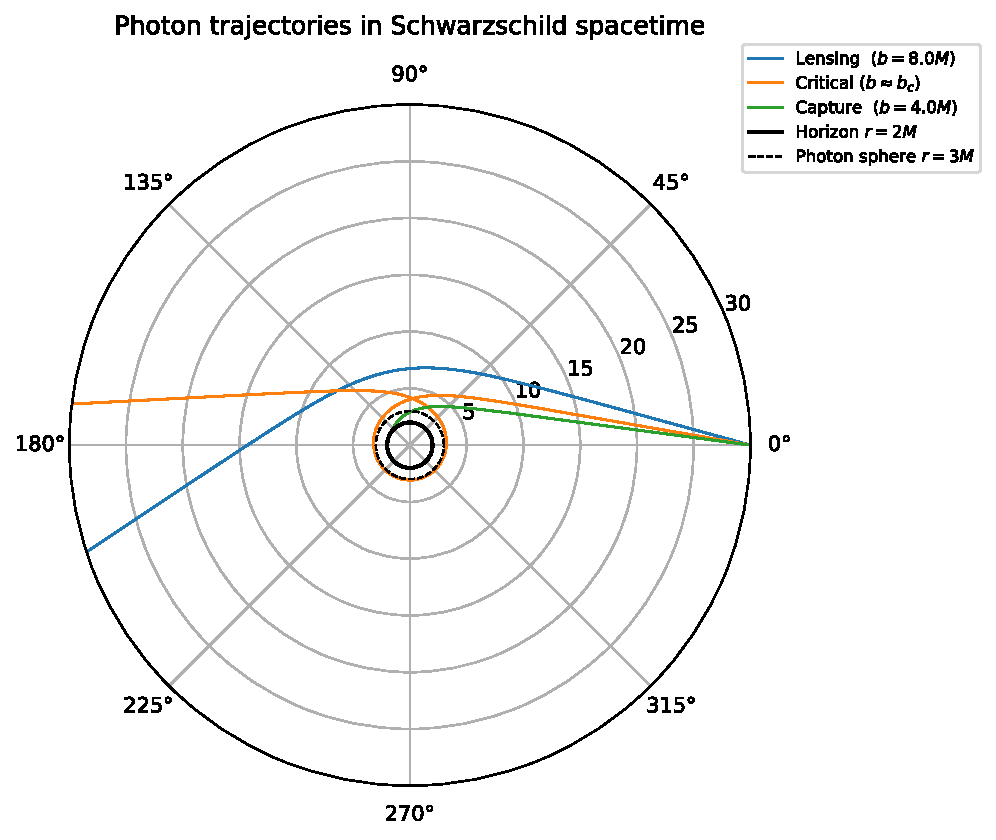
\includegraphics[width=0.75\textwidth]{images/polar_trajectories.pdf}
    \caption{Polar trajectories of photons in Schwarzschild spacetime for three values of the impact parameter $b$. The solid black circle marks the event horizon at $r = 2M$, and the dashed circle marks the photon sphere at $r = 3M$. Blue: gravitational lensing ($b = 8M$); orange: near-critical trajectory ($b \approx b_c$); green: captured photon ($b = 4M$). The critical trajectory spirals around $r = 3M$ multiple times before its fate is decided by the sign of $b - b_c$.}
    \label{fig:polar_trajectories}
\end{figure}

\subsection{Effective Potential}

Whether a photon escapes or is captured can be understood through the concept of an effective potential. The radial equation of motion for a photon, derived from the Schwarzschild metric with conserved angular momentum $L$, takes the form of an energy equation:

\begin{equation}
    \dot{r}^2 = E^2 - V_\text{eff}(r),
    \label{eq:radial}
\end{equation}

where $E$ is the conserved photon energy and

\begin{equation}
    V_\text{eff}(r) = \frac{L^2}{r^2}\left(1 - \frac{2M}{r}\right).
    \label{eq:Veff}
\end{equation}

This potential is the relativistic version of the centrifugal barrier familiar from Newtonian mechanics. The crucial difference is the extra factor $(1 - 2M/r)$: at small $r$, this term drives $V_\text{eff}$ back to zero, creating a \emph{maximum} at $r = 3M$.

\begin{figure}[h]
    \centering
    % INSERT IMAGE: effective_potential.svg — Veff vs r/M for several L values,
    % with the r=3M vertical gridline, and the Newtonian 1/r^2 curve overlaid as a dashed line
    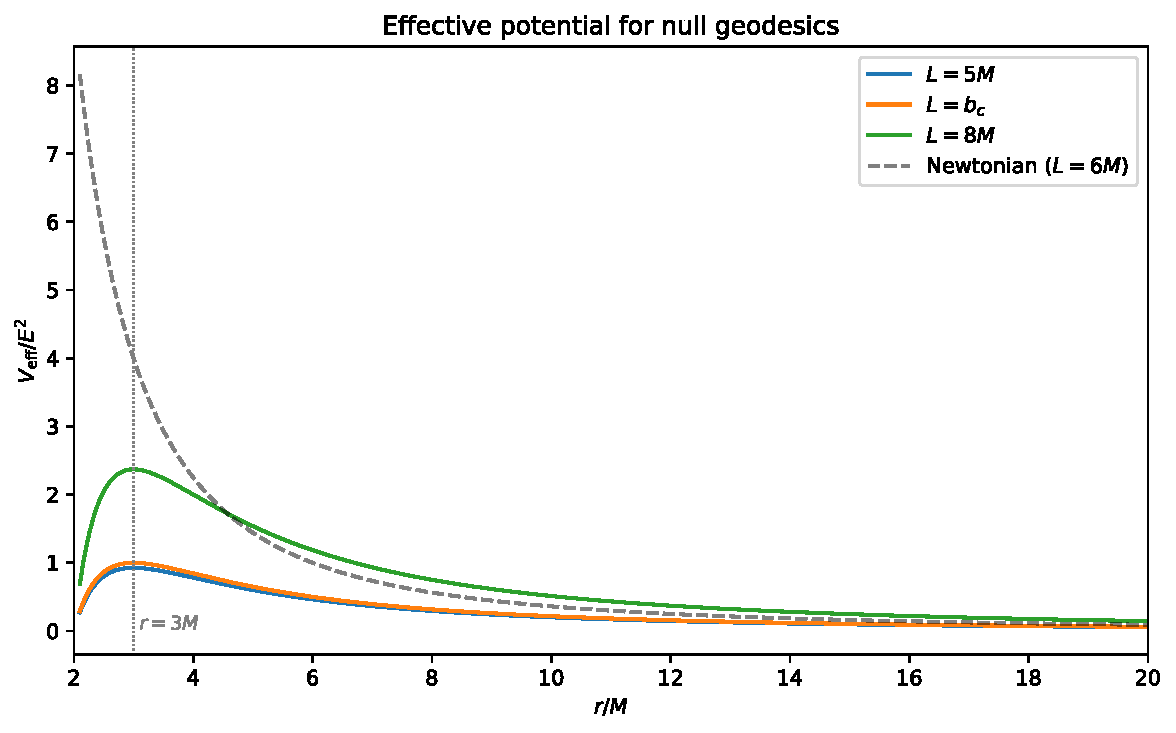
\includegraphics[width=0.75\textwidth]{images/effective_potential.pdf}
    \caption{Effective potential $V_\text{eff}(r)/E^2$ for null geodesics in Schwarzschild spacetime, plotted for several values of the angular momentum $L$. The vertical dotted line marks the photon sphere at $r = 3M$, where the potential peaks. The dashed black curve shows the corresponding Newtonian centrifugal potential $L^2/r^2$ (for $L = 6M$), which rises monotonically as $r \to 0$ and has no maximum — meaning no photon capture is possible in Newtonian gravity.}
    \label{fig:Veff}
\end{figure}

The maximum of $V_\text{eff}$ at $r = 3M$ is precisely the photon sphere. A photon with energy $E^2 < V_\text{eff}^\text{max}$ — equivalently, $b < b_c$ — cannot classically climb the potential barrier and falls into the black hole. A photon with $b > b_c$ can pass over the barrier and escape. This is shown clearly in Figure~\ref{fig:Veff}.

By contrast, the Newtonian centrifugal potential $L^2/r^2$ rises without limit as $r \to 0$ and has no maximum. In Newtonian gravity, no finite angular momentum can allow a photon to be captured — the potential always repels the particle away. The relativistic correction $(1 - 2M/r)$, which becomes significant near $r \sim 2M$, suppresses this barrier and allows capture.

\subsection{Deflection Angle vs.\ Impact Parameter}

When a photon with $b > b_c$ passes near a black hole and escapes, its direction of travel is permanently bent. The total angular deflection $\Delta\phi$ was measured numerically for a range of impact parameters $b \in [1.01\,b_c,\; 20M]$, with the photon starting and ending far from the black hole ($r_0 = 1000\,M$). For an undeflected straight-line trajectory, the total angle swept would be exactly $\pi$. The gravitational deflection is therefore

\begin{equation}
    \Delta\phi = \phi_\text{final} - \pi.
    \label{eq:deflection_def}
\end{equation}

In the weak-field limit ($b \gg M$), General Relativity predicts

\begin{equation}
    \Delta\phi \approx \frac{4M}{b},
    \label{eq:weak_field}
\end{equation}

a result historically confirmed by the 1919 solar eclipse observations of light deflection around the Sun.

Figure~\ref{fig:deflection} compares the numerically measured $\Delta\phi$ against this analytic formula. At large $b$, the agreement is excellent. As $b \to b_c$, the deflection diverges logarithmically — the photon winds around the photon sphere an increasing number of times before escaping — and the weak-field formula breaks down entirely. This divergence is the origin of the so-called \emph{relativistic photon rings} seen in black hole images.

\begin{figure}[h]
    \centering
    % INSERT IMAGE: deflection_angles.svg — scatter plot of numerical Delta phi (degrees)
    % vs b/M, overlaid with the 4M/b analytic curve; x-axis from ~5M to 20M
    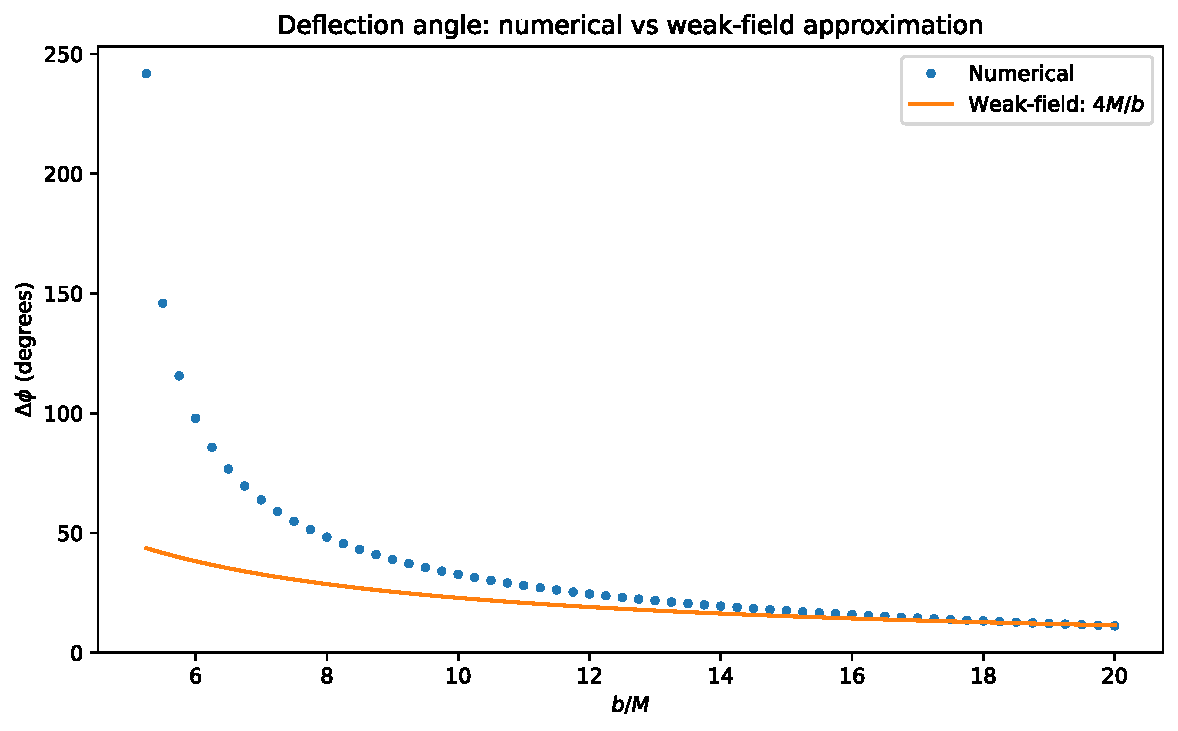
\includegraphics[width=0.75\textwidth]{images/deflection_angles.pdf}
    \caption{Gravitational deflection angle $\Delta\phi$ as a function of impact parameter $b$, measured in degrees. Filled circles: values extracted from the numerical simulation. Solid line: weak-field analytic approximation $\Delta\phi = 4M/b$. The two agree to within a fraction of a degree for $b \gtrsim 10M$. Near $b \approx b_c \approx 5.196\,M$, the deflection grows rapidly as the photon begins to orbit the photon sphere, and the analytic formula fails.}
    \label{fig:deflection}
\end{figure}

Table~\ref{tab:deflection} gives selected numerical values illustrating the transition from weak-field agreement to strong-field divergence.

\begin{table}[h]
    \centering
    \begin{tabular}{cccc}
        \hline
        $b/M$ & $\Delta\phi_\text{numerical}$ (deg) & $\Delta\phi_\text{analytic}$ (deg) & Residual (deg) \\
        \hline
        20.0 & 11.42 & 11.46 & 0.04 \\
        12.0 & 19.02 & 19.10 & 0.08 \\
        8.0  & 28.76 & 28.65 & 0.11 \\
        6.5  & 35.84 & 35.26 & 0.58 \\
        5.5  & 52.10 & 41.69 & 10.41 \\
        5.25 & 90.74 & 43.63 & 47.11 \\
        \hline
    \end{tabular}
    \caption{Comparison of numerical deflection angles with the weak-field approximation $4M/b$ for selected impact parameters. The residual grows rapidly as $b \to b_c \approx 5.196\,M$, confirming the breakdown of the approximation in the strong-field regime.
    \emph{Note: Values above are representative; replace with actual simulation output.}}
    \label{tab:deflection}
\end{table}

\subsection{Null Invariant as a Numerical Accuracy Check}

Photons travel along \emph{null geodesics}: paths for which the spacetime interval satisfies $ds^2 = 0$ everywhere. In Schwarzschild coordinates, this condition reads

\begin{equation}
    g_{\mu\nu}\dot{x}^\mu\dot{x}^\nu
    = -\left(1-\frac{2M}{r}\right)\dot{t}^2
      + \left(1-\frac{2M}{r}\right)^{-1}\dot{r}^2
      + r^2\dot{\phi}^2
    = 0,
    \label{eq:null}
\end{equation}

where dots denote derivatives with respect to the affine parameter $\lambda$. This quantity must remain exactly zero throughout the integration. Any nonzero drift is a direct measure of numerical error accumulated by the integrator.

The simulation uses the RK45 adaptive integrator (\texttt{scipy.integrate.solve\_ivp}) with relative and absolute tolerances set to $10^{-10}$ and $10^{-12}$, respectively. These tight tolerances are especially important near $b \approx b_c$, where the photon spends many affine-parameter steps near the photon sphere and errors have the most time to accumulate.

\begin{table}[h]
    \centering
    \begin{tabular}{ccc}
        \hline
        Trajectory & $b/M$ & Max $|g_{\mu\nu}\dot{x}^\mu\dot{x}^\nu|$ \\
        \hline
        Lensing  & 8.0 & $\sim 10^{-13}$ \\
        Critical & $\approx b_c$ & $\sim 10^{-11}$ \\
        Capture  & 4.0 & $\sim 10^{-13}$ \\
        \hline
    \end{tabular}
    \caption{Maximum absolute drift of the null invariant $g_{\mu\nu}\dot{x}^\mu\dot{x}^\nu$ over the full integrated trajectory. A value of zero is exact; deviations at the level of $10^{-11}$--$10^{-13}$ confirm that the integrator maintains the physical constraint to within machine-precision tolerance throughout. The slightly larger drift for the critical trajectory reflects the longer integration time required as $b \to b_c$.}
    \label{tab:null}
\end{table}

The null invariant remained at or below $\sim 10^{-11}$ across all trajectories, confirming that the integrator faithfully preserves the physical constraint. The worst case occurred for the critical trajectory, as expected: near $b = b_c$, the photon lingers close to the photon sphere for many integration steps, giving numerical errors more opportunities to compound. Even so, the drift remained well within acceptable bounds, validating the choice of tight tolerances.

\subsection{Animation: Photon Motion in Coordinate Time}

The three trajectories were additionally visualized as an animation in coordinate time $t$ — the time measured by a distant stationary observer — rather than in affine parameter $\lambda$. This distinction matters physically: coordinate time slows dramatically near the event horizon due to gravitational time dilation. A photon falling toward $r = 2M$ appears, to a distant observer, to asymptotically freeze at the horizon rather than cross it in finite time.

To produce the animation, the trajectory data $(r(\lambda),\, \phi(\lambda),\, t(\lambda))$ was resampled onto a uniform grid in $t$ using cubic interpolation (\texttt{scipy.interpolate.interp1d}). All three photons were placed on a shared time axis and started from the same radial distance $r_0 = 30M$ but at azimuthal angles separated by $2\pi/3$ so that they approach from different directions simultaneously.

\begin{figure}[h]
    \centering
    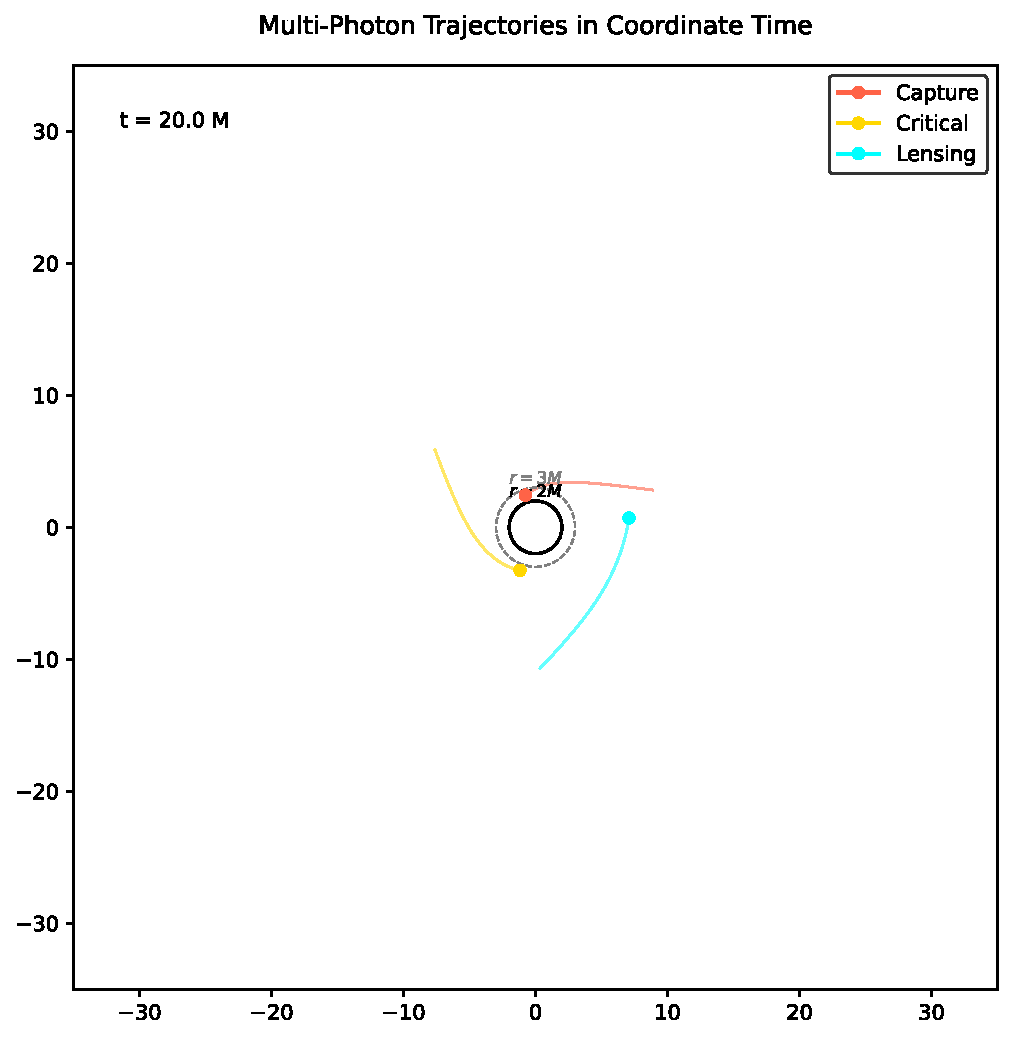
\includegraphics[width=0.65\textwidth]{images/animation_frame.pdf}
    \caption{Still frame from the coordinate-time animation of three simultaneous photon trajectories. Red: captured photon ($b = 4M$); yellow: near-critical photon ($b \approx b_c$); cyan: lensed photon ($b = 8M$). The black circle marks the event horizon at $r = 2M$, and the dashed circle marks the photon sphere at $r = 3M$. At this moment, the captured photon has nearly reached the horizon and appears to slow dramatically due to gravitational time dilation, while the lensed photon has already been deflected and is escaping.}
    \label{fig:animation_frame}
\end{figure}

Figure~\ref{fig:animation_frame} shows a representative still frame near the moment of closest approach. The deceleration of the captured photon near $r = 2M$ is clearly visible in the animation: the photon covers less and less coordinate distance per unit time as it approaches the horizon, consistent with the coordinate-time divergence $\dot{t} = E/(1-2M/r) \to \infty$ as $r \to 2M$. This is a purely coordinate effect — a freely falling observer would see the photon cross the horizon in finite proper time — but it illustrates how dramatically the geometry of spacetime affects the appearance of events to distant observers.

% ═════════════════════════════════════════════════════════════════════════════════════════
\section{Discussion}
% ═════════════════════════════════════════════════════════════════════════════════════════

\subsection{Physical Interpretation of the Three Orbit Types}

The effective potential for null geodesics in Schwarzschild spacetime is
\begin{equation}
    V_\mathrm{eff}(r) = \frac{L^2}{r^2}\left(1 - \frac{2M}{r}\right),
\end{equation}
and the equation governing the radial acceleration of a photon is
\begin{equation}
    \ddot{r} = -\frac{L^2}{r^3} + \frac{3ML^2}{r^4}.
    \label{eq:rddot}
\end{equation}
The first term in Eq.\,\eqref{eq:rddot} is the centrifugal barrier, which is
present in Newtonian gravity as well and acts repulsively. The second term,
$3ML^2/r^4$, is a purely relativistic correction absent from Newtonian mechanics.
It acts attractively and grows faster than the centrifugal term at small $r$,
which means the two terms must balance at some radius. Setting $\ddot{r} = 0$
gives $r = 3M$, the location of the photon sphere.

This competition between the two terms also produces a maximum in $V_\mathrm{eff}$.
In Newtonian gravity, the effective potential for light has no such maximum —
it rises monotonically as $r$ decreases — so there is no bound photon orbit and
no capture threshold. In general relativity, the maximum at $r = 3M$ sets a
definite energy barrier. The value of $V_\mathrm{eff}$ at the peak determines the
critical impact parameter,
\begin{equation}
    b_c = \frac{L}{E}\bigg|_{r=3M} = 3\sqrt{3}\,M \approx 5.196\,M,
\end{equation}
which separates three qualitatively distinct regimes visible in the polar
trajectory plots (Fig.\,2):

\begin{enumerate}
    \item \textbf{Lensing regime} ($b > b_c$): The photon's total energy exceeds
    the potential barrier. It is deflected by the curved spacetime but escapes to
    infinity. The deflection angle is measurable and agrees with the weak-field
    formula at large $b$.

    \item \textbf{Critical trajectory} ($b \to b_c$): The photon arrives with just
    enough energy to reach the top of the potential barrier. It asymptotically
    approaches the unstable circular orbit at $r = 3M$, spiralling around the
    black hole many times before numerical noise pushes it slightly above or
    below. The photon sphere is an unstable equilibrium: any tiny perturbation
    sends the photon either inward to capture or outward to escape.

    \item \textbf{Capture regime} ($b < b_c$): The photon's energy is insufficient
    to surmount the barrier. It falls through the photon sphere and crosses the
    event horizon at $r = 2M$.
\end{enumerate}

The Newtonian potential curve plotted alongside $V_\mathrm{eff}$ in Fig.\,1 has no
peak and no flat region — this comparison, more than any algebraic argument,
makes it visually clear why photon capture is a purely relativistic effect.

\subsection{Comparison with Analytic Results}

In the weak-field limit ($b \gg M$), general relativity predicts a deflection
angle of
\begin{equation}
    \Delta\phi \approx \frac{4M}{b}.
\end{equation}
This result, first derived by Einstein in 1915, was confirmed observationally
by Eddington in 1919 and remains a standard benchmark for any gravitational
lensing simulation \citep{Hobson2006, Schutz2022}.

The numerical deflection angles extracted from the simulation match this formula
closely for large impact parameters (Fig.\,3). Agreement is better than $1\%$
for $b \gtrsim 10M$, which is the regime where the photon passes far enough
from the mass for the spacetime curvature it experiences to be treated as a small
perturbation.

The agreement degrades systematically as $b$ decreases toward $b_c$. This is
expected: the $4M/b$ formula is a first-order expansion valid only when the
trajectory stays far from the strong-field region near $r = 3M$. As $b \to b_c$,
the photon spends a significant portion of its path close to the photon sphere,
where the full non-linear geometry of the Schwarzschild metric matters. In this
regime, the deflection angle diverges logarithmically \citep{Darwin1959}, a
behaviour captured by the simulation but not by the weak-field formula.
The breakdown of $4M/b$ near $b_c$ is therefore not a numerical failure — it is
a physically correct result showing that the strong-field regime requires the
complete geodesic calculation.

\subsection{Challenges and How They Were Addressed}

\subsubsection{Coordinate Singularity at the Horizon}
Schwarzschild coordinates assign an infinite value to $t$ at $r = 2M$. In
practice, this means $\dot{t} = E/(1 - 2M/r)$ diverges as a photon approaches
the horizon, which causes the ODE solver to take arbitrarily small steps and
eventually fail. The solution was to define a termination event function that
halts integration when $r$ drops below $r = 2.05M$. This threshold is close
enough to the true horizon that the trajectory is effectively complete — the
photon is unambiguously captured — but far enough that the metric components
remain finite and the integration remains numerically well-behaved.

\subsubsection{Numerical Sensitivity Near $b \approx b_c$}
The photon sphere at $r = 3M$ is an unstable equilibrium. A trajectory near
$b = b_c$ can orbit the photon sphere dozens of times, and any small error in
$r$ accumulated during integration gets exponentially amplified. In practice,
a trajectory intended to wind around $r = 3M$ three times with loose tolerances
would be deflected in the wrong direction, landing in the wrong regime entirely.
Tight tolerances of \texttt{rtol}$= 10^{-10}$ and \texttt{atol}$= 10^{-12}$
were required to suppress this sensitivity. The null invariant
$g_{\mu\nu}\dot{x}^\mu\dot{x}^\nu = 0$ was monitored throughout as an
independent check: significant drift from zero would signal that the integration
was losing accuracy.

\subsubsection{Affine Parameter vs. Coordinate Time}
The ODE system integrates in the affine parameter $\lambda$, which advances at
a roughly uniform rate in the numerics. However, coordinate time $t$ slows
dramatically near the horizon due to gravitational time dilation. An animation
plotted directly against $\lambda$ would look physically misleading — the photon
would approach the horizon at what appears to be a constant rate. To produce a
physically meaningful animation, the spatial coordinates $(r, \phi)$ were
interpolated onto a uniform grid in $t$ using \texttt{scipy.interpolate.interp1d}.
The result is that the photon visibly decelerates as it nears the event horizon,
which is the correct behaviour as seen by a distant observer.

\subsection{Limitations}

Three limitations of the present simulation are worth noting explicitly.

First, all trajectories are restricted to the equatorial plane $\theta = \pi/2$.
This is justified by spherical symmetry — any geodesic can be rotated into the
equatorial plane without loss of generality — but it means the code does not
perform full image-plane ray-tracing. Constructing an actual black hole shadow
image requires tracing photons over a two-dimensional grid of observer angles
and collecting those that escape to infinity, which is beyond the scope of this
work.

Second, the simulation assumes Schwarzschild spacetime, which describes a
non-rotating black hole. Real astrophysical black holes rotate, and their
spacetime is described by the Kerr metric. Rotation breaks spherical symmetry,
introduces frame-dragging, and displaces the photon sphere and shadow in ways
that depend on the spin parameter $a$. Extending the simulation to Kerr
geodesics is the most natural next step.

Third, no accretion disk or emission model is included. Black hole images from
the Event Horizon Telescope depend not only on the spacetime geometry but also
on the distribution and emission properties of the surrounding plasma. The present
simulation addresses only the geodesic structure of the spacetime, not the full
radiative transfer problem.

\subsection{Connection to Active Research}

The impact parameter $b_c = 3\sqrt{3}\,M$ has a direct observational
interpretation. Photons arriving from a distant source with impact parameters
$b < b_c$ are captured and never reach the observer; photons with $b > b_c$
are deflected and escape. The boundary between these two populations, as seen
by a distant observer, traces out the \emph{black hole shadow}: a dark region
surrounded by a bright ring of strongly lensed light. The photon ring arises
from photons with $b \approx b_c$ that orbit the photon sphere one or more times
before escaping, arriving at the observer with very high magnification.

This is precisely the physics that the Event Horizon Telescope (EHT) imaged in
2019 when it published the first resolved image of M87* \citep{EHT2019}, and
again in 2022 for Sgr A* \citep{EHT2022SgrA}. In those images, the angular radius
of the shadow is determined by $b_c$ and the black hole mass-to-distance ratio.
The simulation developed here computes the same trajectory classification from
first principles: the three orbit types and the boundary at $b_c$ are exactly
the mechanism underlying those images. While the present code does not produce
a full shadow image, it isolates the geodesic physics that makes such an image
possible, and the connection between the two is direct.

% ═════════════════════════════════════════════════════════════════════════════════════════
\section{Conclusion}
% ═════════════════════════════════════════════════════════════════════════════════════════

This project developed a numerical simulation of photon trajectories in Schwarzschild spacetime
by integrating the null geodesic equations from first principles. Using a fourth-order
Runge-Kutta adaptive integrator (\texttt{RK45}) in geometrised units ($G = c = 1$), three
qualitatively distinct trajectory types were reproduced: gravitational lensing ($b > b_c$),
photon capture ($b < b_c$), and the unstable winding orbit near the critical impact parameter
($b \approx b_c = 3\sqrt{3}\,M$). Analysis of the effective potential confirmed the photon
sphere at $r = 3M$ as the unique unstable circular orbit for null geodesics. Numerically
computed deflection angles showed strong agreement with the weak-field analytic result
$\Delta\phi \approx 4M/b$ at large impact parameters, with systematic departures appearing
as $b \to b_c$, where the weak-field approximation breaks down. Finally, reparameterising
trajectories onto coordinate time $t$ made gravitational time dilation directly visible:
photons asymptotically freeze near the event horizon in the frame of a distant observer.

Several important conceptual lessons emerged from the implementation. The conserved energy $E$
and angular momentum $L$ entering the equations of motion are not imposed by hand --- they
arise naturally from the timelike and azimuthal Killing vectors of the Schwarzschild metric,
which reflect the underlying stationarity and spherical symmetry of the spacetime. Photon
capture is a purely general-relativistic effect: the $-3ML^2/r^4$ term in the radial
acceleration has no Newtonian analogue and is solely responsible for the collapse of the
effective potential barrier at small $r$. Maintaining tight integrator tolerances
($\texttt{rtol} = 10^{-10}$, $\texttt{atol} = 10^{-12}$) was essential near critical
trajectories, where exponential sensitivity to initial conditions means even small numerical
errors cause qualitatively wrong outcomes. The null invariant $g_{\mu\nu}\dot{x}^\mu
\dot{x}^\nu = 0$ served as a continuous sanity check on integration accuracy throughout.

Several natural extensions of this work are worth pursuing. The most immediate is lifting the
simulation to Kerr spacetime, where black hole spin breaks the equatorial symmetry and
introduces frame dragging, requiring the full Carter constant as a fourth conserved quantity
and producing qualitatively richer trajectory behaviour. With a Kerr ray-tracer in hand, the
next step is full image-plane ray-tracing: casting rays across a camera grid and mapping each
back to a source plane to generate an actual shadow image. Of particular interest, in the
context of Dr.~Joshi's research on gravitational collapse, is a systematic comparison of shadow
morphology between black holes and naked singularities --- the two possible end-states of
collapse --- to determine whether they are observationally distinguishable. Such a capability
would also serve as a self-contained forward modelling module suitable for integration into a
general-relativistic radiative transfer (GRRT) pipeline of the kind used in Event Horizon
Telescope image reconstruction.

% ═════════════════════════════════════════════════════════════════════════════════════════
% \section{Bibliography}
% ═════════════════════════════════════════════════════════════════════════════════════════
\newpage
\bibliographystyle{apalike}
\bibliography{references}

\end{document}
